%!TEX root = ../Thesis.tex
\chapter{Experimental results}
\label{sec:results}

%--------------------------------------------------------------------------------
\clearpage
\section{Initial investigation: WAFFLE experiment}
\label{sec:waffle}

Placeholder

%--------------------------------------------------------------------------------
\clearpage
\section{Addendum: Key results and lessons learned}
\label{sec:waffle_addendum}

Placeholder

%--------------------------------------------------------------------------------
\clearpage
\section{Introduction to second study: \newline 
{\O}sterild Balconies experiment}
\label{sec:balcony_intro}

\begin{comment}
Necessary to measure at zero elevation angle
Avoid influence from terrain and vegetation
Similar to offshore conditions
Scope of NEWA project fit well into this thesis
\end{comment}

%--------------------------------------------------------------------------------
\clearpage
\section{Minute-Scale Wind Speed Forecasting Using Scanning Lidar Inflow Measurements}
\label{sec:balcony_paper}

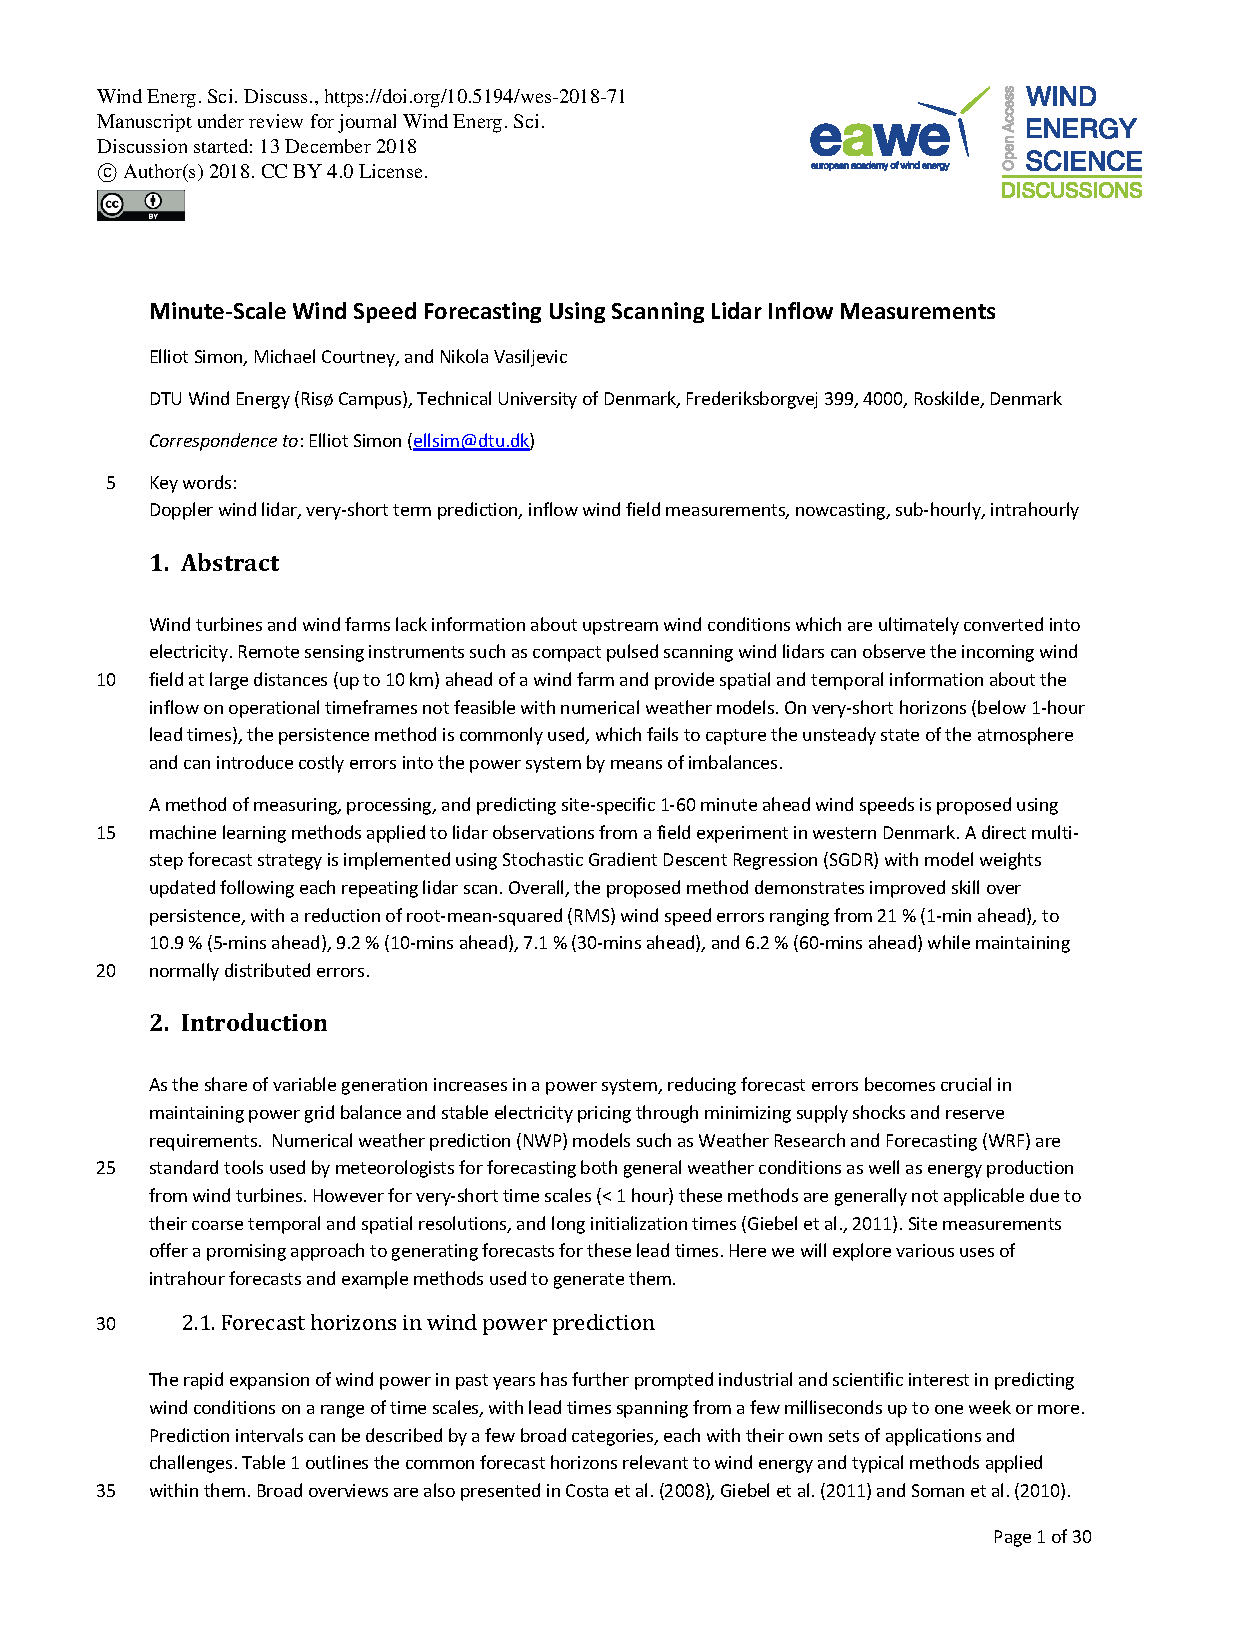
\includepdf[pages=-]{papers/Balcony_paper_WESD.pdf}

%--------------------------------------------------------------------------------
\clearpage
\section{Addendum 1: Weather front event}
\label{sec:balcony_addendum1}

This section expands upon an oral presentation titled "Lidars Lifted: The {\O}sterild Balconies Experiment" given at the 97th American Meteorological Society (AMS) conference in Seattle (\cite{simon_lidars_lifted_2017}).

During the first phase of the Balconies experiment while the scanning lidars were deployed at 50 m above ground level (AGL),
a weather event was encountered with a potentially high impact for an operational wind turbine or wind farm.

At approximately 7PM on the 6th of June 2016, the arrival of a cold front drastically changed the wind regime at the test site. Although there was not a significant wind speed ramp, the wind directions of the two air masses were diametrically opposed. The result was a near instant 180 degree shift in wind direction (from 130 to 310 degrees) as the 


\begin{figure}[htbp]
    \centering
        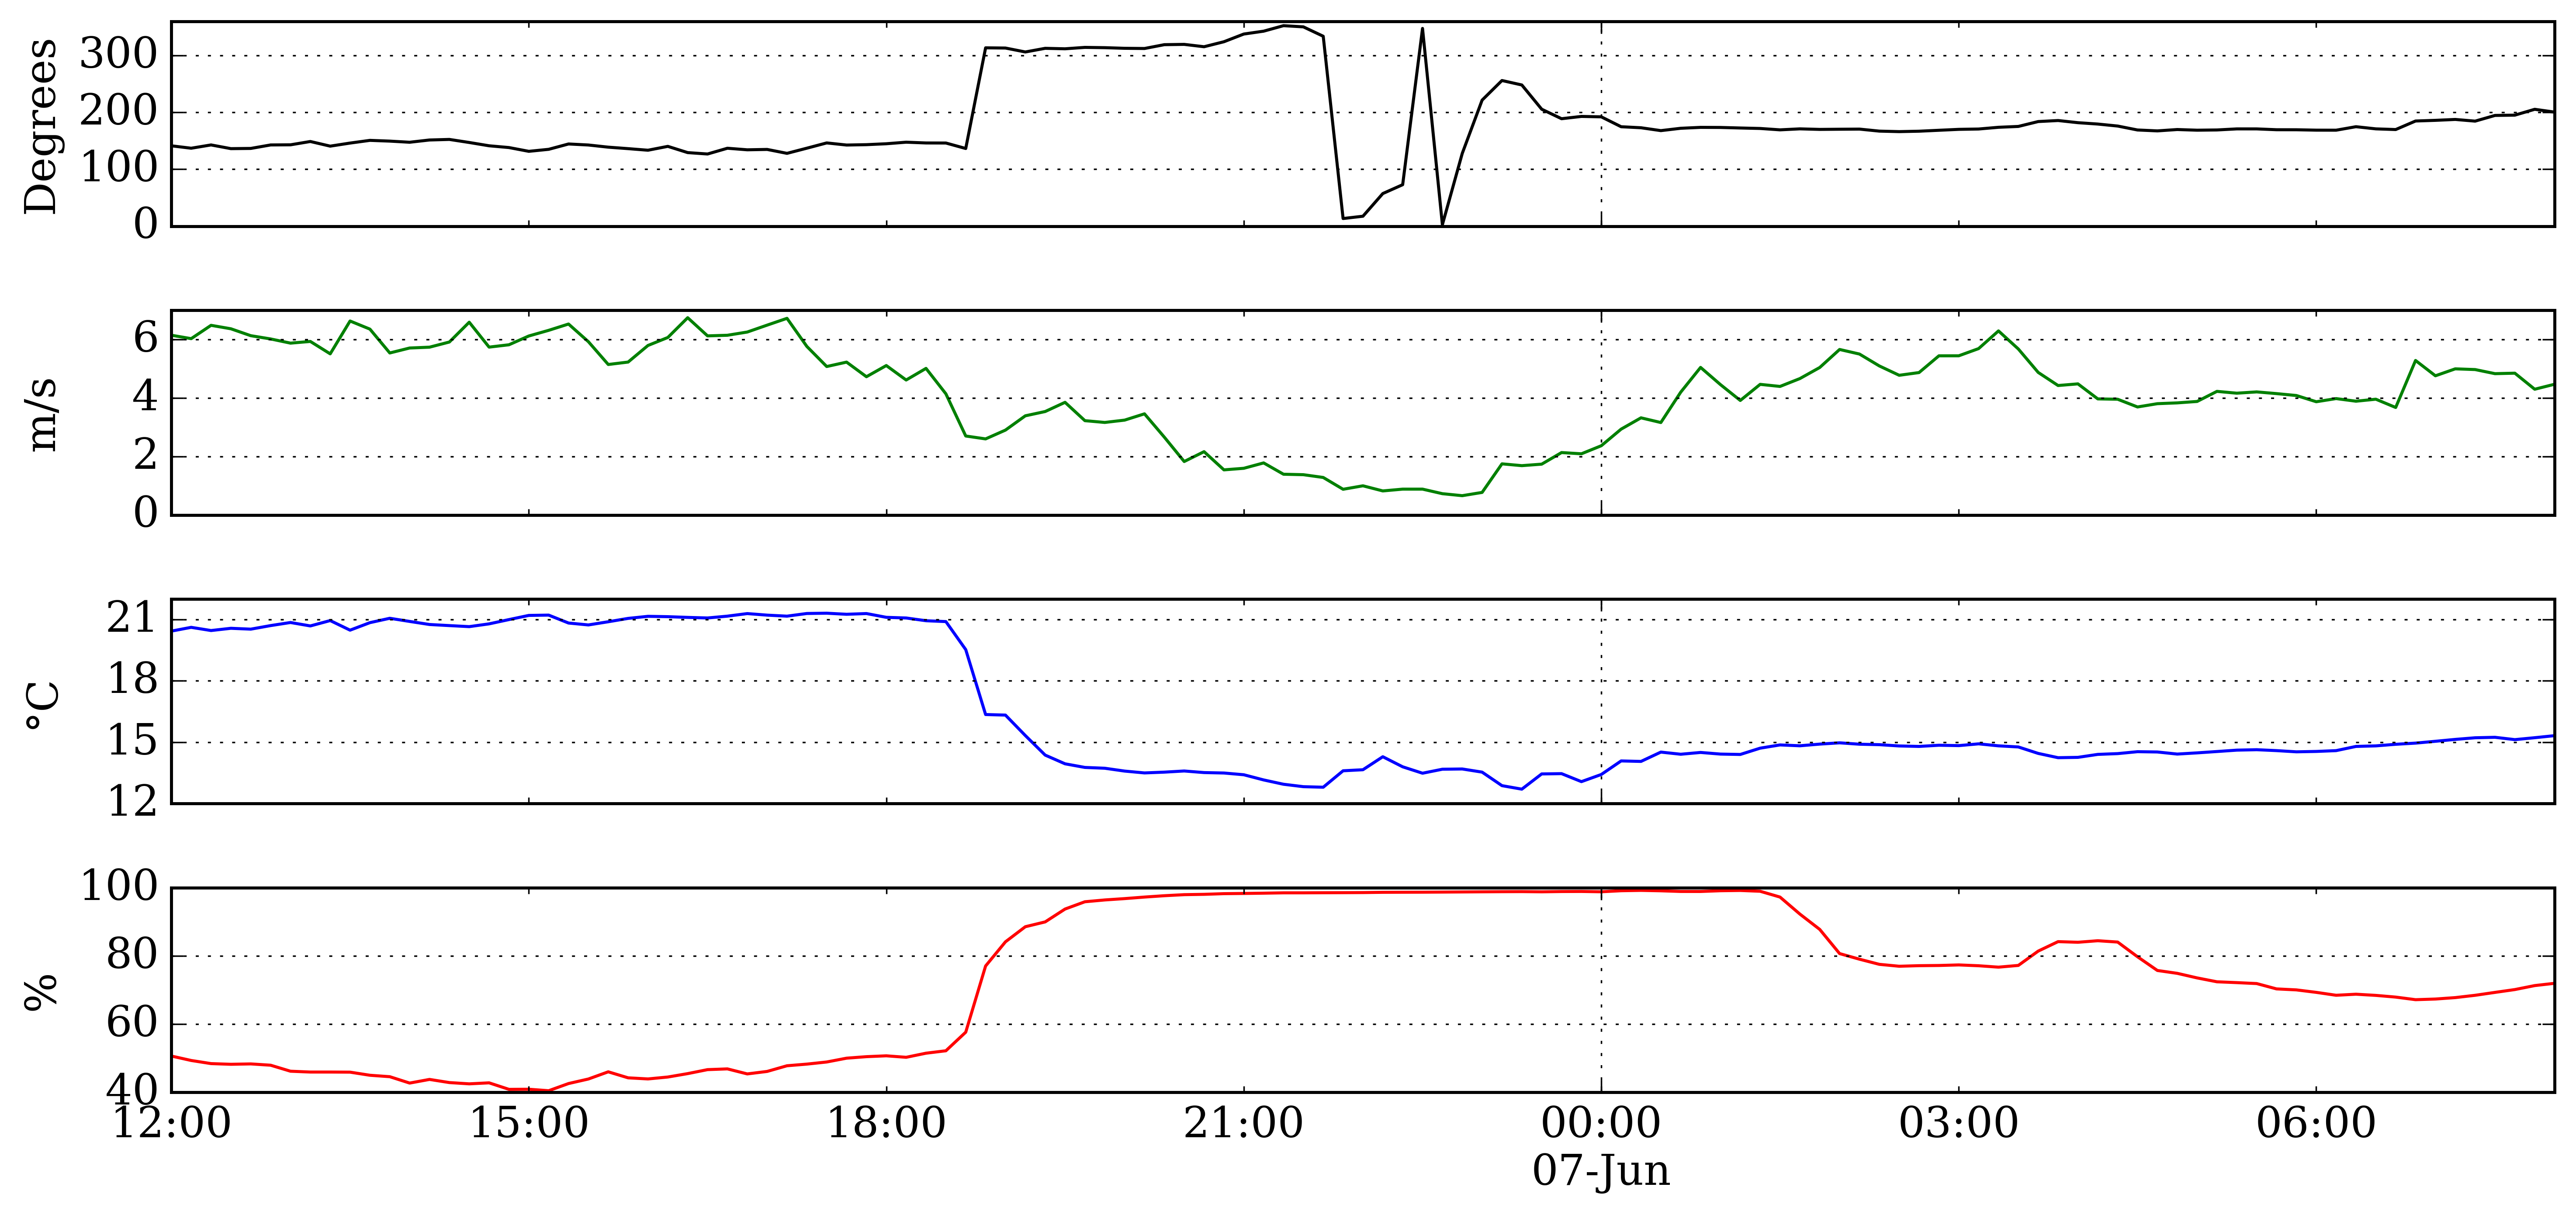
\includegraphics[width=1.0\textwidth]{graphics/intro/balcony-addendum/balcony-front-mast.png}
    \caption{Mast measurements during a passing cold front at {\O}sterild test center on June 6-7, 2016.
    Top panel: Wind direction at 40 m AGL. Second panel: Wind speed at 40 m AGL. Third panel: Temperature at 37 m AGL. Bottom panel: Relative humidity at 7 m AGL}
    \label{fig:balcony-front-mast}
\end{figure}


















%--------------------------------------------------------------------------------
\clearpage
\section{Addendum 2: Key results and lessons learned}
\label{sec:balcony_addendum2}

Placeholder


%--------------------------------------------------------------------------------
\clearpage
\section{Introduction to third study: LASCAR experiment}
\label{sec:lascar_intro}

Placeholder


%--------------------------------------------------------------------------------
\clearpage
\section{Minute-Scale Wind Vector Forecasting Using Scanning Lidar Inputs to a Convolutional LSTM Neural Network}
\label{sec:lascar_paper}

Placeholder for LASCAR paper
%\includepdf[pages=-]{papers/LASCAR_paper.pdf}

%--------------------------------------------------------------------------------
\clearpage
\section{Addendum: Key results and lessons learned}
\label{sec:lascar_addendum}

Placeholder